\section{Simulations and Performance Analysis}
In this section we describe the implementation of our simulator and discuss some performance measurements acquired using this tool. We also describe features that should be added to the simulator to support more realistic experiments. We conclude with a discussion of good parameter selection based on our observations using the simulator.

\subsection{Simulation Design}
To assess the expected overhead introduced by Boomerang we implemented a custom discrete-time simulator that emulates the behavior of Bitcoin nodes (software clients) running Boomerang. Time in the simulation is measured in epochs; at every epoch a series of events occurs that advances the state of the system in some (usually) deterministic way. Our simulator supports the following behavior to closely resemble Boomerang:
\begin{enumerate}
	\item Nodes enter and exit the network at random times. 
	\item Nodes make new transactions using configuration-specificed parameters $W$ and $D$ at a random rate $\pi$.
	\item Nodes generate cover traffic at a random rate $\sigma$.
	\item Nodes manage their internal address address books according the protocol described in section \ref{sec:design}.
\end{enumerate}

In addition, the simulation dynamically computes the following performance metrics:
\begin{enumerate}
	\item Average number of ``computations'' done per node (i.e., the number of public-key encryption operations to encode a transaction).
	\item Total and average message latency from the start to end of a circuit for single and every message, respectively.
	\item Node forwarding throughput (messages/s).
	\item Number of completed messages (transactions and cover messages) vs the number of in-progress messages.
	\item Average number of transaction broadcast retries per node.
\end{enumerate}

The parameters for a particular simulation are specified via a YAML configuration file which is parsed using the Java-based JYaml library \cite{jyaml}. An example configuration file which creates a simulation with $N = 100$ nodes, $D = 6$, $W = 2$, and cover and transaction generation rates uniformly distributed between $[1, 5000]$ and $[1, 7500]$ epochs (i.e., the most granular unit of time).

\begin{lstlisting}
simTime: 2500
numNodes: 100
enterRate: 750
exitRate: 750
gridHeight: 10000
gridWidth: 10000
chaffGenRate: 5000
txGenRate: 7500
circuitWidth: 2
circuitDepth: 6
retryLimit: 7500
buffSize: 10
mixDelay: 50
pktSize: 1024
initialAddressSize: 250
validNodeTransmitReq: 50
addressBookSize: 1000
seed: 256
outfileprefix: "config-out"
path: "."
genMatrices: false
keepInMemory: false
\end{lstlisting}

The {\tt genMatrices} and {\tt keepInMemory} flags are used to ensure that the Java heap space isn't exhausted from memory leaks by storing all of the events generated by the simulation at each time epoch. To run the simulation with 8GB of heap space on the example configuration listed above, which is stored in a local file {\tt config.yaml}, one would run the following command:

\begin{center}
{\small \tt java -cp ./jyaml-1.3.jar:. -Xmx8g Boomerang config.yaml}
\end{center}

\subsection{Performance Metrics and System Parameters}
Using our simulation, we performed a series of small and large experiments; the properties and simulation results for a subset of such experiments are summarized in Tables \ref{tab:experiments} and \ref{tab:sim-results}, respectively\footnote{Due to physical memory limitations and the initial single-threaded nature design of our simulator, we could not conduct experiments beyond $N \approx 25000$. We will address this shortcoming in our simulation design for future work.}. Contrary to what one might originally anticipate, there is no clear relationship between the number of messages (cover traffic and encoded transactions) generated and average number of transaction retries. As more messages flood the network, one would expect that the message flow to be expedited since mix node buffers fill up quicker, leading to a higher average number of forwarded messages. As a result, one might also naively expect that the likelihood of transaction retries would decrease because transactions would propogate through their respective circuits much quicker. However, the flow of traffic in the network is dependent on many variables, including the rate of cover and transaction generation, the distribution of node selection during circuit formation, the mix buffer size, and the random mix delay. Formulating a markovian model for the flow of traffic throughout the network is beyond the scope of this work, so we just note that more experiments should be conducted to gain a better understanding of how these system parameters interact with one another. 

We can, however, state with relative certainty that the performance overhead of the Boomerang scheme is tightly coupled to $W$, $D$, and the rate at which cover traffic and new encoded transactions generation ($\sigma$ and $\pi$, respectively). Furthermore, given our anonymity analysis and these performance results, it is clear that we wish to maximize $D$ (circuit depth) and minimize $W$ (circuit width - or the number of independent circuits) so as to reduce the overall work performed by a node while also improving anonymity. However, observe that with few independent circuits of larger depth, the likelihood that a transaction needs to be re-transmitted is increased. This result appeals to intuition since a larger number of hops will ultimately increase the overall message latency.

An illustration of cover and transaction messages flowing through the network during the entire duration of Experiment \#1 is shown in Figure \ref{fig:flow}, and a series of smaller windows during which this information is captured is shown in Figure \ref{fig:small-flow}. As expected, the flow of messages appears to be uniformly distributed across all nodes, even when analyzed in small time windows. 

To summarize, we recommend that $D$ is maximized, $W$ is minimized, and $\sigma$ is maximized subject to node computational limitations and the expected congestion of the network. Choosing an appropriate value for $\sigma$ should be tied to the expected transaction generation rate $\pi$, which is ultimately controlled by the users, i.e., it is not a system parameter. Unfortunately, we do not have the means to estimate this rate, and thus we leave the selection of the system parameters as future work dependent on such an analysis. 

\begin{table*}
\begin{center}
\caption{Subset of experimental parameters explored with the Boomerang simulator.}
\label{tab:experiments}
    \begin{tabular}{|c|c|c|c|c|c|} \hline
    {\bf Experiment \#} & $N$ & $D$ & $W$ & $\sigma_{max}$ & $\pi_{max}$ \\ \hline
    1 & 50     & 6 & 2 & 5000 & 7500 \\ 
    2 & 100    & 6 & 2 & 5000 & 7500 \\ 
    3 & 150    & 6 & 2 & 5000 & 7500 \\ 
    4 & 200    & 6 & 2 & 5000 & 7500 \\ 
    5 & 250    & 6 & 2 & 5000 & 7500 \\ 
    6 & 1000   & 6 & 2 & 5000 & 7500 \\ 
    7 & 10000  & 6 & 2 & 5000 & 7500 \\ 
    8 & 50     & 8 & 1 & 5000 & 15000 \\ 
    9 & 100    & 8 & 1 & 5000 & 15000 \\ 
    10 & 150   & 8 & 1 & 5000 & 15000 \\ 
    11 & 200   & 8 & 1 & 5000 & 15000 \\ 
    12 & 250   & 8 & 1 & 5000 & 15000 \\ 
    13 & 1000  & 8 & 1 & 5000 & 15000 \\ 
    14 & 10000 & 8 & 1 & 5000 & 15000 \\ 
    \hline
    \end{tabular}
\end{center}
\end{table*}

\begin{table*}
\begin{center}
\caption{Simulation results gathered from the experiment configurations listed in Table \ref{tab:experiments}. Since message latency is not a goal of Boomerang (i.e., the timeliness of transaction broadcasts is not of critical importance), this measurement is omitted for brevity. All simulations were run for a }
\label{tab:sim-results}
% chaff, transaction, num forwarded, number of retries
    \begin{tabular}{|c|c|c|c|c|} \hline
    {\bf Experiment \#} & {\bf Avg. Chaff Generated} & {\bf Avg. Transactions Encoded} & {\bf Avg. Forwarded Messages} & {\bf Avg. Retries} \\ \hline
    1  & 18.47 & 8.5 & 1.11 & 0.15 \\
    2  & 46.63 & 19.01 & 20.84 & 1.08 \\
    3  & 58.23 & 24.36 & 29.78 & 1.41 \\
    4  & 30.09 & 13.46 & 3.32 & 0.27 \\
    5  & 72.45 & 30.48 & 39.67 & 1.80 \\
    6  & 35.83 & 15.49 & 5.21 & 0.32 \\
    7  & 36.57 & 16.0 & 4.88 & 0.33 \\
    8  & 7.27 & 3.54 & 0.0 & 0.09 \\
    9  & 20.36 & 10.33 & 2.10 & 0.83 \\
    10 & 26.56 & 13.47 & 4.27 & 1.11 \\
    11 & 31.69 & 16.54 & 6.99 & 1.4 \\
    12 & 35.91 & 18.18 & 7.37 & 1.55 \\
    13 & 15.77 & 6.48 & 0.0 & 0.16 \\
    14 & 16.22 & 6.65 & 0.05 & 0.17 \\
    \hline
    \end{tabular}
\end{center}
\end{table*}

\begin{figure*}[ht!]
\begin{center}
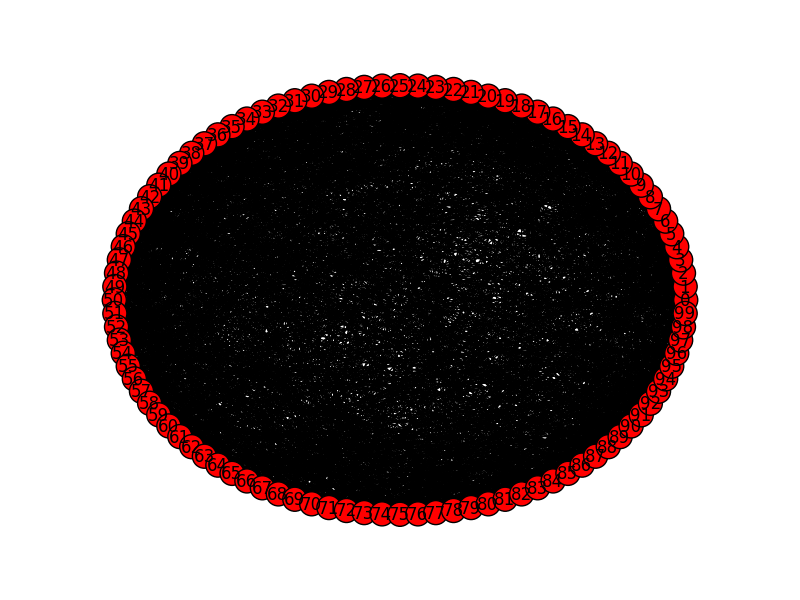
\includegraphics[scale=0.5]{./images/sim1_completedMessage_complete.png}
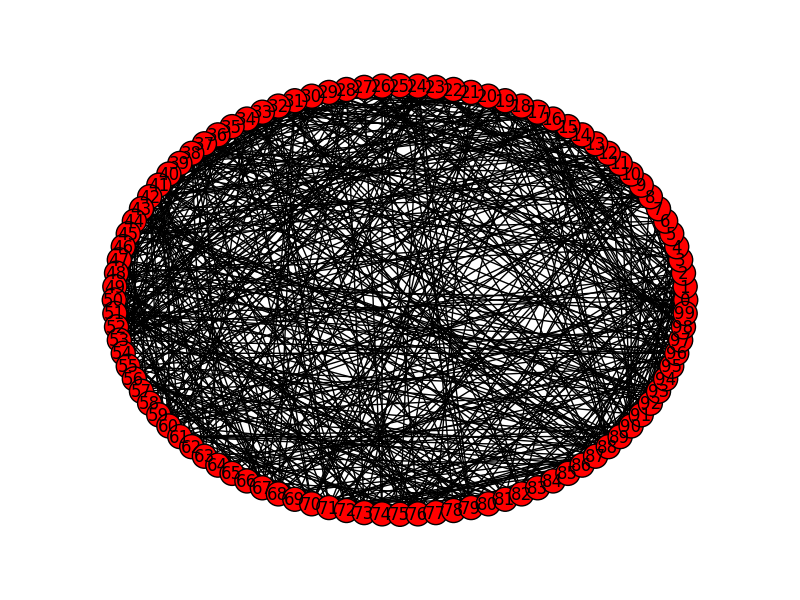
\includegraphics[scale=0.5]{./images/sim1_completedMessage_tx.png}
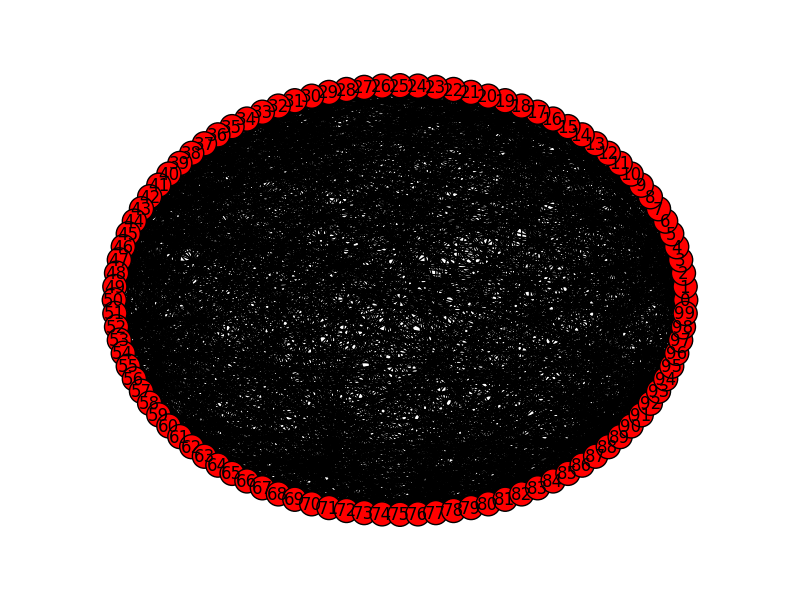
\includegraphics[scale=0.5]{./images/sim1_completedMessage_chaff.png}
\caption{The top figure shows the flow of both dummy messages and forwarded transactions from Experiment \#1, the middle figure shows only the transaction messages, and the bottom figure shows the cover traffic. Nodes have directed edges between them if some message was sent between them during the lifetime of the simulation. The coverage of nodes is clearly uniformly distributed, as desired.}
\label{fig:flow}
\end{center}
\end{figure*}

\begin{figure*}
\begin{center}
\begin{tabular}{ccc}
  \num\putindeepbox[2pt]{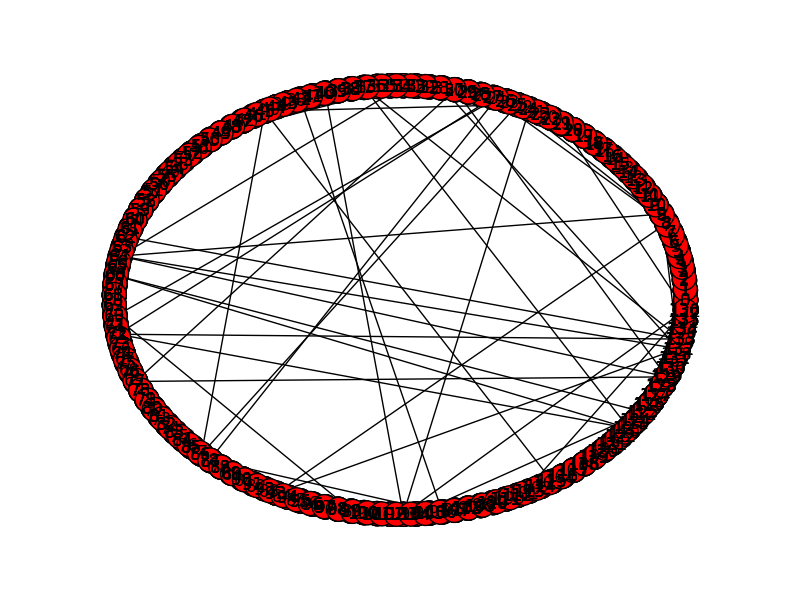
\includegraphics[scale=0.25]{images/sim2_1_complete.png}}
    & \num\putindeepbox[2pt]{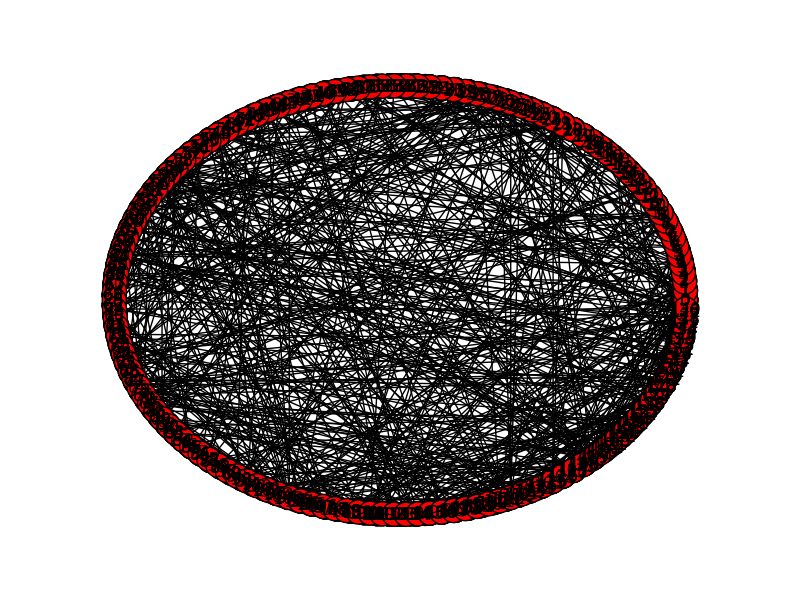
\includegraphics[scale=0.25]{images/sim2_2_complete.png}} 
    & \num\putindeepbox[2pt]{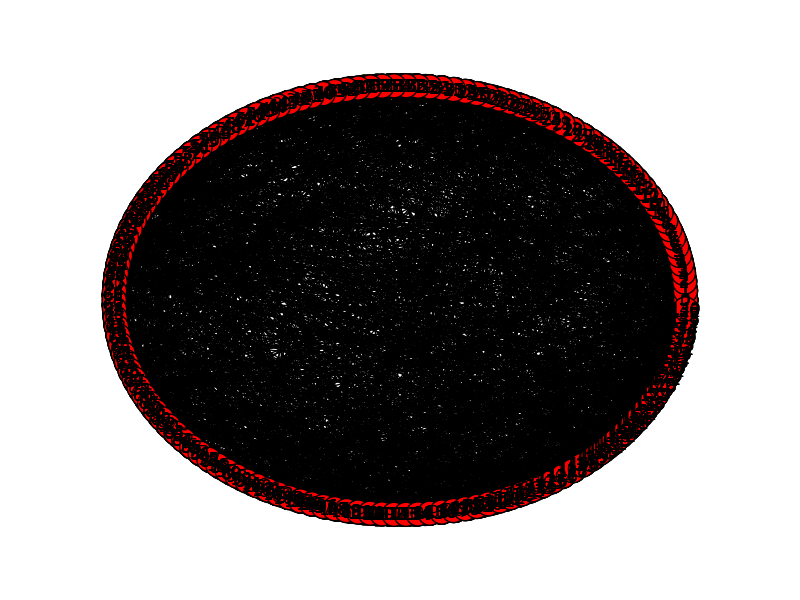
\includegraphics[scale=0.25]{images/sim2_3_complete.png}} \\
  
  \num\putindeepbox[2pt]{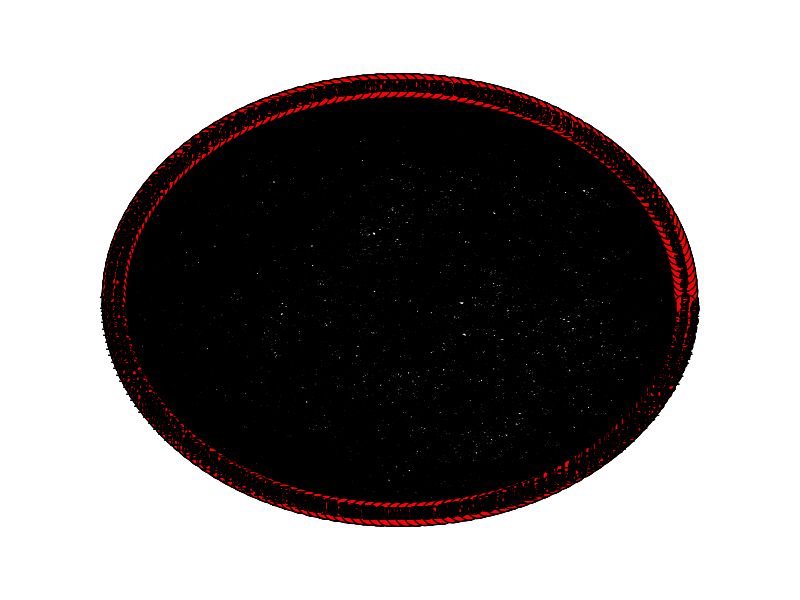
\includegraphics[scale=0.25]{images/sim2_4_complete.png}} 
  & \num\putindeepbox[2pt]{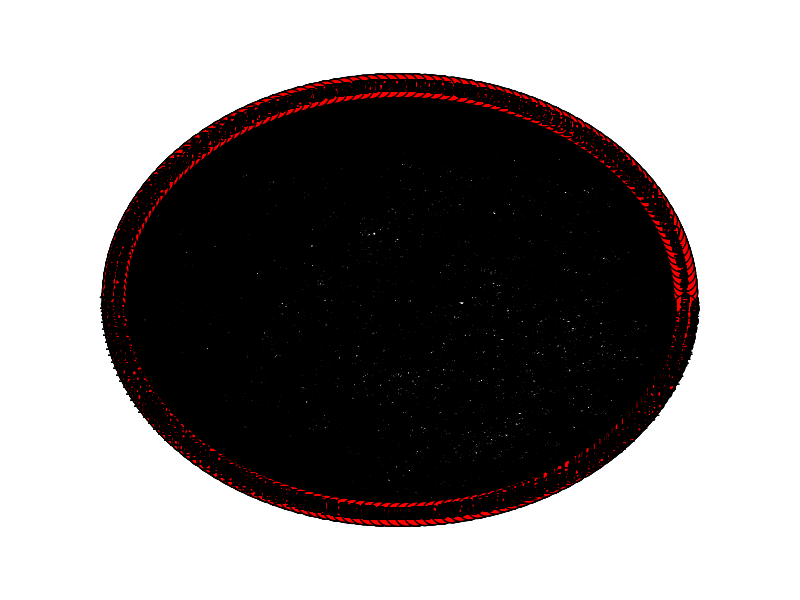
\includegraphics[scale=0.25]{images/sim2_5_complete.png}} 
  & \num\putindeepbox[2pt]{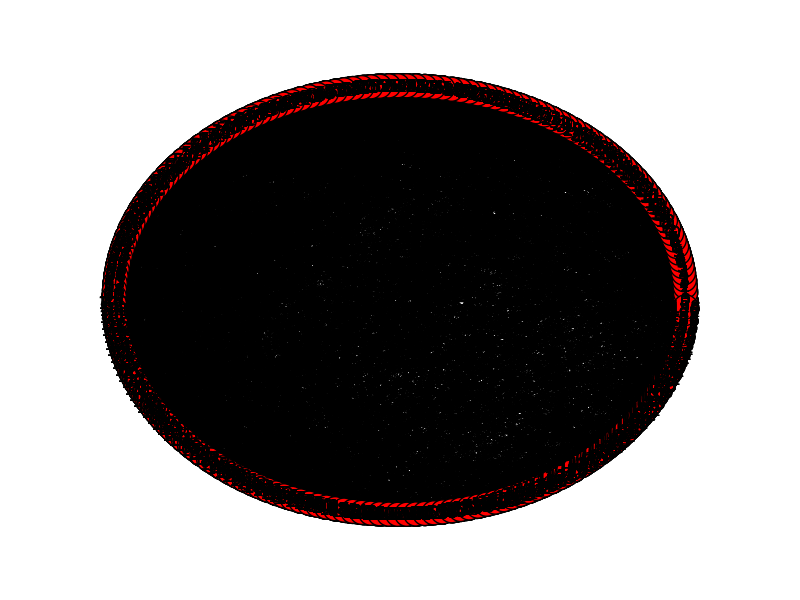
\includegraphics[scale=0.25]{images/sim2_6_complete.png}}\\
  
  \num\putindeepbox[2pt]{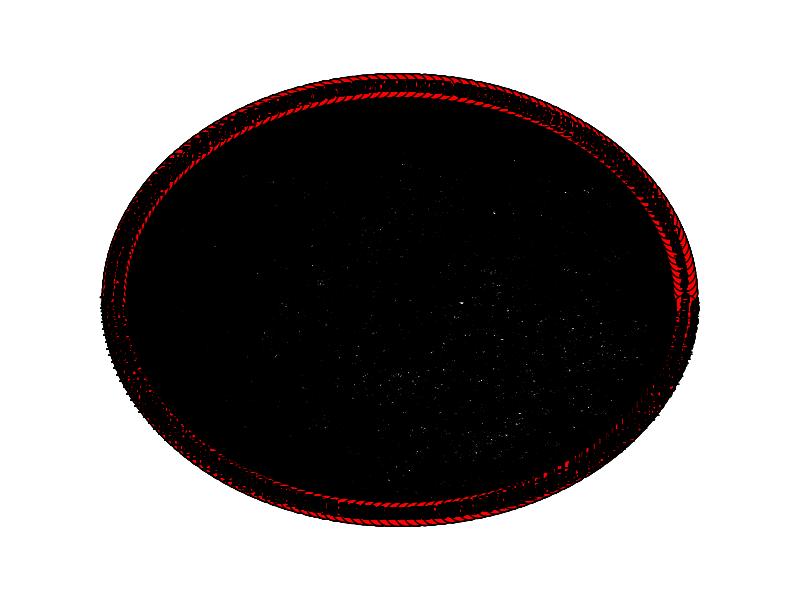
\includegraphics[scale=0.25]{images/sim2_7_complete.png}}
    & \num\putindeepbox[2pt]{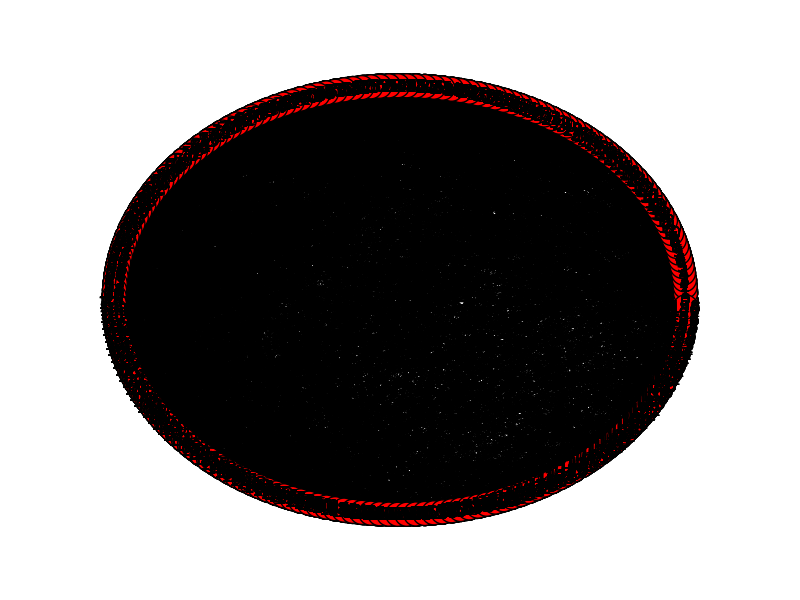
\includegraphics[scale=0.25]{images/sim2_8_complete.png}} 
    & \num\putindeepbox[2pt]{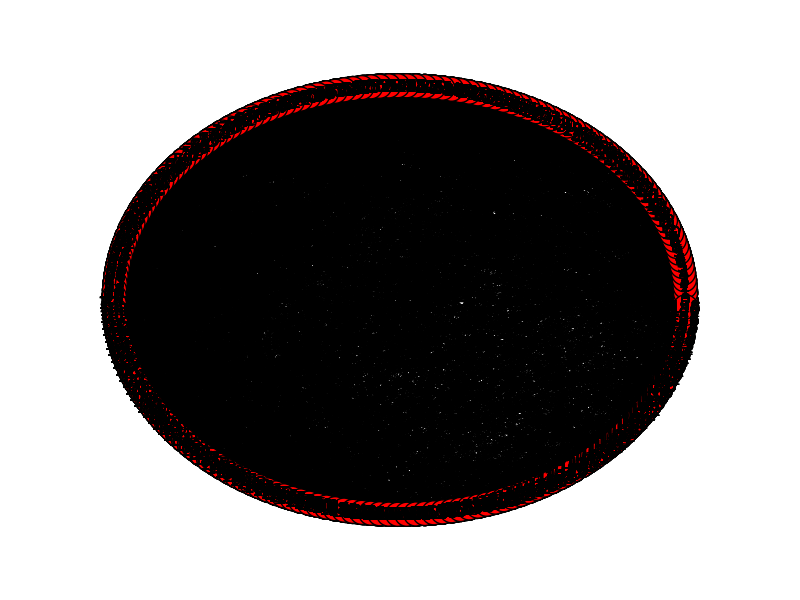
\includegraphics[scale=0.25]{images/sim2_9_complete.png}} \\
  
  \num\putindeepbox[2pt]{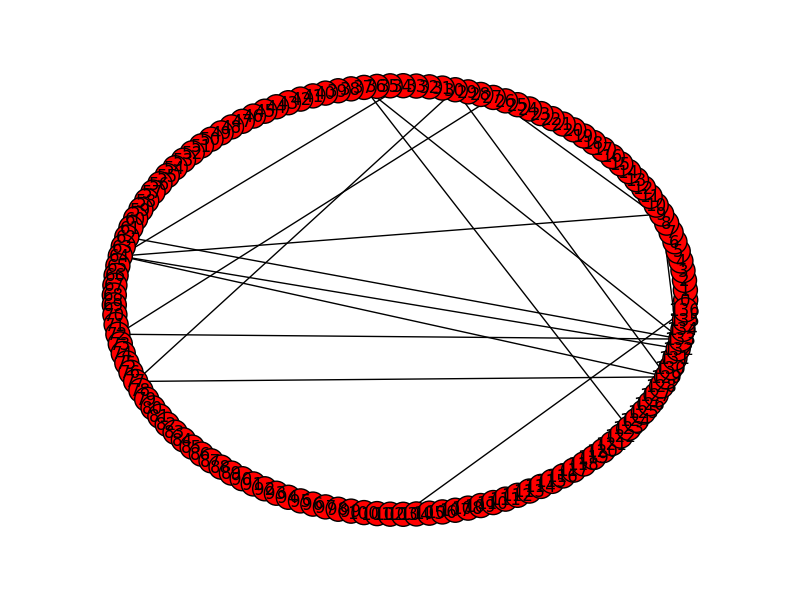
\includegraphics[scale=0.25]{images/sim2_10_complete.png}} 
   & \num\putindeepbox[2pt]{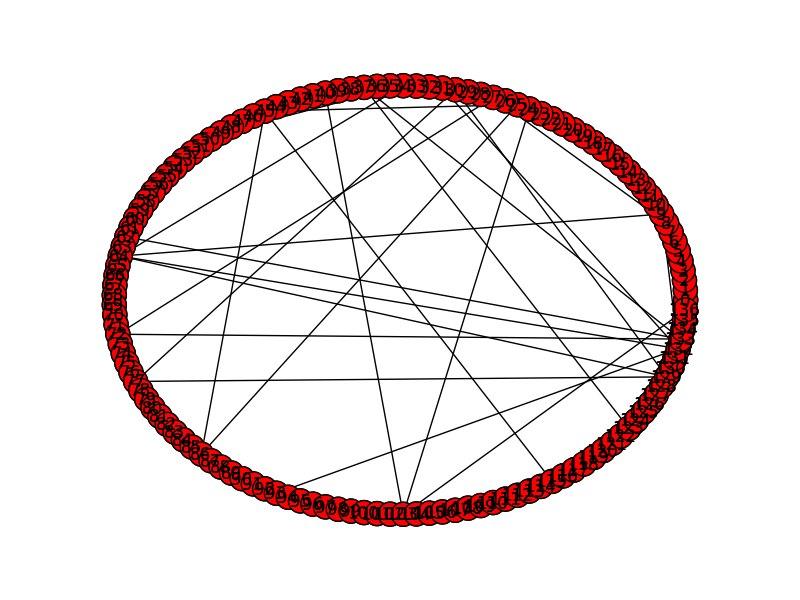
\includegraphics[scale=0.25]{images/sim2_11_complete.png}} 
    & \num\putindeepbox[2pt]{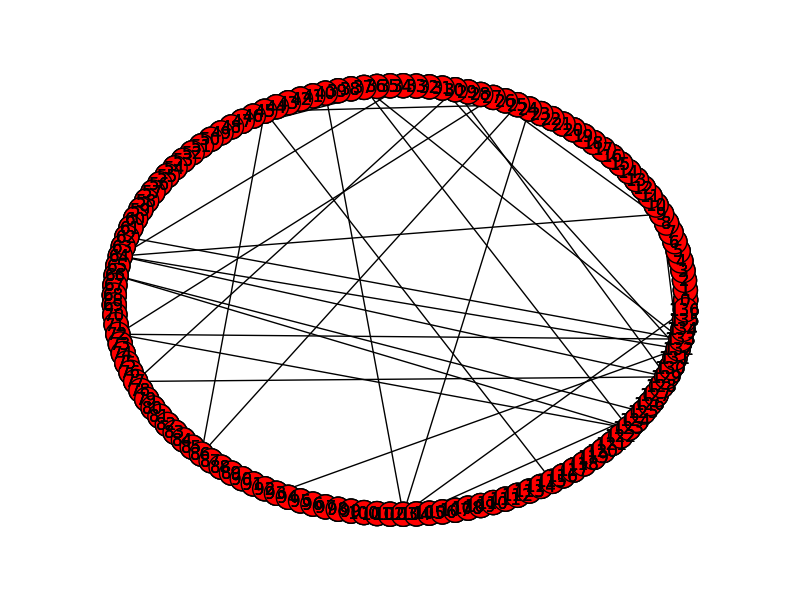
\includegraphics[scale=0.25]{images/sim2_12_complete.png}}\\
\end{tabular}
\end{center}
\caption{Time series evolution of message flow in the Boomerang network. The flow of messages becomes quite uniform as the number of generated messages increases, which can be seen by the increased density of message flow and uniform message trajectories. The reduction in messages near the end is an artifact of the simulator in that messages stop being generated when the simulation time approaches the specified time limit.}
\label{fig:small-flow}
\end{figure*}

% cover traffic generation rate (random variable)
% mix buffer delay (random variable)
% circuit length (fixed)
% mix buffer size (fixed)
% encoded transaction size

